
\chapter{Least squares and Singular Values}
\label{sec:leastsquaresSVD}
\index{Least squares}

Consider the linear algebraic equation $L(x)=v$, where $L \colon U\stackrel{\text{linear}}{-\!\!\!-\!\!\!\longrightarrow}W$ and $v\in W$ are known while $x$ is unknown. As we have seen, this system may have 
one solution, no solutions, or infinitely many solutions.  
But if $v$ is not in the range of $L$ there will {\itshape never} be any solutions for $L(x)=v$.
\vspace{-.1cm}
\begin{center}
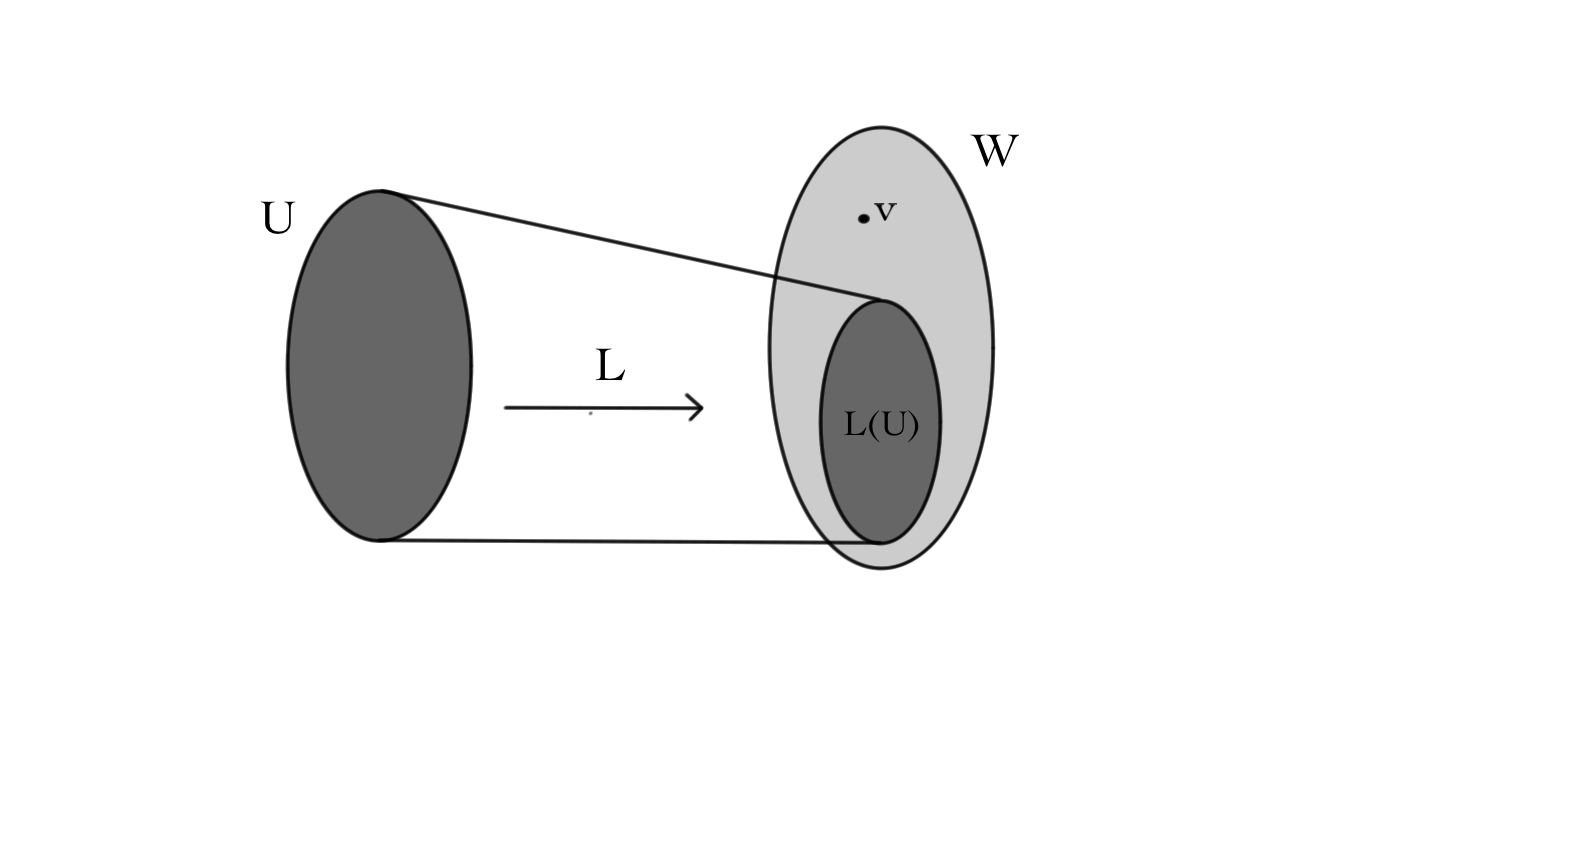
\includegraphics[scale=.24]{notinimage.jpg}
\end{center} 
\vspace{-1.8cm}
However, for many applications we do not need an exact solution of the system; instead, we may only need the best approximation possible.  

\begin{quote}
``My work always tried to unite the Truth with the Beautiful, but when I had to choose one or the other, I usually chose the Beautiful.'' 

\vspace{-2mm}
\hspace{7cm}-- Hermann Weyl.
\end{quote}

If the vector space $W$ has a notion of lengths of vectors, we can try to find $x$ that minimizes $||L(x)-v||$.
\begin{center}
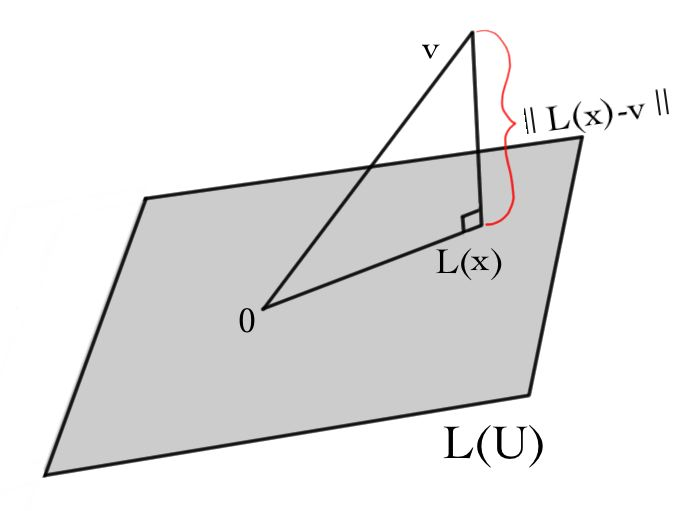
\includegraphics[scale=.24]{minimize.jpg}
\end{center} 
This method has many applications, such as when trying to fit a (perhaps linear) function to a ``noisy'' set of observations.  For example, suppose we measured the position of a bicycle on a racetrack once every five seconds.  Our observations won't be exact, but so long as the observations are right on average, we can figure out a best-possible linear function of position of the bicycle in terms of time.

Suppose $M$ is the matrix for the linear function $L:U \to W$ in some bases for $U$ and $W$. The vectors~$v$ and~$x$ are represented by column vectors $V$ and $X$ in these bases.  Then we need to approximate
\[
MX-V\approx 0\, .
\]

Note that if $\dim U=n$ and $\dim W=m$ then $M$ can be represented by an $m\times n$ matrix and $x$ and $v$ as vectors in $\Re^n$ and $\Re^m$, respectively. Thus, we can write $W=L(U)\oplus L(U)^\perp$.  Then we can uniquely write $v=v^\parallel + v^\perp$, with $v^\parallel \in L(U)$ and $v^\perp \in L(U)^\perp$.  



Thus we should solve $L(u)=v^\parallel$.  In components, $v^\perp$ is just $V-MX$, and is the part we will eventually wish to minimize.  

In terms of $M$, recall that $L(V)$ is spanned by the columns of $M$.  (In the standard basis, the columns of $M$ are $Me_1$, 
$\ldots$, $Me_n$.)  Then $v^\perp$ must be perpendicular to the columns of $M$.  \textit{i.e.}, $M^T(V-MX)=0$, or
\[
M^TMX = M^TV.
\]
Solutions of $M^TMX = M^TV$ for $X$ are called \emph{least squares}\index{Least squares!solutions} solutions to $MX=V$.  
Notice that any solution $X$ to $MX=V$ is a least squares solution.  However, the converse is often false.  In fact, the equation $MX=V$ may have no solutions at all, but still have least squares solutions to $M^TMX = M^TV$.

Observe that since $M$ is an $m\times n$ matrix, then $M^T$ is an $n\times m$ matrix.  Then $M^TM$ is an $n\times n$ matrix, and is symmetric, since $(M^TM)^T=M^TM$.  Then, for any vector $X$, we can evaluate $X^TM^TMX$ to obtain a number.  This is a very nice number, though!  It is just the length $|MX|^2 = (MX)^T(MX)=X^TM^TMX$.

%\href{\webworkurl ReadingHomework25/1/}{Reading homework: problem 25.1}
\Reading{LeastSquares}{1}

Now suppose that $\ker L=\{0\}$, so that the only solution to $MX=0$ is $X=0$. (This need not mean that $M$ is invertible because $M$ is an $n\times m $ matrix, so not necessarily square.) 
However the square matrix $M^TM$ {\itshape is} invertible. To see this, suppose there was a vector $X$ such that 
$M^T M X=0$. Then it would follow that $X^T M^T M X = |M X|^2=0$. In other words the vector $MX$ would have zero length, so could only be the zero vector. But we are assuming that $\ker L=\{0\}$ so $MX=0$ implies $X=0$. Thus the kernel of $M^TM$ is $\{0\}$ so this matrix is invertible.
So, in this case, the least squares solution (the $X$ that solves $M^TMX=MV$) is unique, and is equal to 
\[
X = (M^TM)^{-1}M^TV.
\]
In a nutshell, this is the least squares method:

\begin{itemize}
\item Compute $M^TM$ and $M^TV$.
\item Solve $(M^TM)X=M^TV$ by Gaussian elimination.
\end{itemize}


\begin{example}
Captain Conundrum\index{Captain Conundrum} falls off of the leaning tower of Pisa and makes three (rather shaky) measurements of his velocity at three different times.

\begin{center}
\begin{tabular}{c|c}
$t$ s & $v $ m/s \\ \hline
$1$ & $11$ \\
$2$ & $19$ \\
$3$ & $31$
\end{tabular}
\end{center}

Having taken some calculus\footnote{In fact, he is a \emph{Calculus Superhero}\index{Calculus Superhero}.}, he believes that his data are best approximated by a straight line
\[
v = at+b.
\]
Then he should find $a$ and $b$ to best fit the data.
\begin{align*}
11 &= a\cdot 1 + b \\
19 &= a\cdot 2 + b \\
31 &= a\cdot 3 + b.
\end{align*}
As a system of linear equations, this becomes:

\[
\begin{pmatrix}
1 & 1 \\
2 & 1 \\
3 & 1 \\
\end{pmatrix}
\colvec{a\\b} \stackrel{?}{=}
\colvec{11\\19\\31}.
\]
There is likely no actual straight line solution, so instead solve $M^TMX=M^TV$.

\[
\begin{pmatrix}
1 & 2 & 3 \\
1 & 1 & 1 \\
\end{pmatrix}
\begin{pmatrix}
1 & 1 \\
2 & 1 \\
3 & 1 \\
\end{pmatrix} \colvec{a\\b}
= 
\begin{pmatrix}
1 & 2 & 3 \\
1 & 1 & 1 \\
\end{pmatrix}
\colvec{11\\19\\31}.
\]
This simplifies to 

\[
\begin{amatrix}{2}
14 & 6 & 142 \\
6 & 3 & 61
\end{amatrix}
\sim
\begin{amatrix}{2}
1 & 0 & 10 \\
0 & 1 & \frac{1}{3}
\end{amatrix}.
\]
Thus, the least-squares fit is the line

\[
v = 10\ t + \frac{1}{3}\, .
\]
Notice that this equation implies that Captain Conundrum accelerates towards Italian soil at 10 m/s$^2$ (which is an excellent
approximation to reality) and that he started at a downward velocity of $\frac13$ m/s (perhaps somebody gave him a shove...)!

\end{example}

\section{Projection Matrices}
We have seen that even if $MX=V$ has no solutions $M^TMX=M^T V$ does have solutions. One way to think about this is, since the codomain of $M$ is the direct sum 
\[ \text{codom M}=\text{ran} M \oplus \ker M^T\] 
there is a unique way to write  $V=V_r+V_k$ with $V_k\in \ker M^T$ and $V_r\in \text{ran }\, M$, and it is clear that $Mx=V$ only has a solution of 
$V\in \text{ran}\, M \Leftrightarrow V_k=0$. If not, then the closest thing to a solution of $MX=V$ is a solution to $MX=V_r$. We learned to find solutions to this in the previous subsection of this book. 

But here is another question, how can we determine what $V_r$ is given $M$ and $V$? The answer is simple; suppose $X$ is a solution to $MX=V_r$. Then
\begin{gather*}  MX=V_r 
\implies M^TMx=M^T V_r 
\implies M^TMx=M^T (V_r + 0) \\
\implies M^TMx=M^T (V_r+V_k)
\implies M^TMx=M^T V 
\implies X=(M^TM)^{-1} M^T V 
\end{gather*}
if indeed $M^TM$ is invertible. Since, by assumption, $X$ is a solution \\
\begin{center}
\shabox{ $M(M^TM)^{-1} M^T\, V =V_r. $}
\end{center}
That is, the matrix which projects $V$ onto its $\text{ran} \, M$ part is $M(M^TM)^{-1} M^T$. 

\begin{example} To project $\colvec{1\\1\\1}$ onto $\spa \left\{    \colvec{ 1\\1\\0}, \colvec{1\\-1\\0 }  \right\} = \text{ran} 
\begin{pmatrix}
 1& 1  \\
1 & -1  \\
0 & 0 
\end{pmatrix}
 $ 
  multiply by the matrix 
 \begin{gather*}
\begin{pmatrix}
 1& 1  \\
1 & -1  \\
0 & 0 
\end{pmatrix}
\left [ 
 \begin{pmatrix}
 1& 1 &0 \\
1 & -1 &0 
\end{pmatrix}
\begin{pmatrix}
 1& 1  \\
1 & -1  \\
0 & 0 
\end{pmatrix}
 \right]^{-1}
 \begin{pmatrix}
 1& 1 &0 \\
1 & -1 &0 
\end{pmatrix}
 \\
=\begin{pmatrix}
 1& 1  \\
1 & -1  \\
0 & 0 
\end{pmatrix}
 \begin{pmatrix}
 2& 0  \\
0 & 2  
\end{pmatrix}^{-1}
 \begin{pmatrix}
 1& 1 &0 \\
1 & -1 &0 
\end{pmatrix} 
\\
=\frac12 \begin{pmatrix}
 1& 1  \\
1 & -1  \\
0 & 0 
\end{pmatrix}
 \begin{pmatrix}
 1& 1 &0 \\
1 & -1 &0 
\end{pmatrix} 
=
\frac12 \begin{pmatrix}
 2 & 0 &0 \\
0 & 2  &0\\
0 & 0 &0
\end{pmatrix}. 
\end{gather*}

This gives 
\[\frac12 \begin{pmatrix}
 2 & 0 &0 \\
0 & 2  &0\\
0 & 0 &0
\end{pmatrix}
\colvec{1\\1\\1 } = \colvec{1\\1\\0} .\]
\end{example}



\section{Singular Value Decomposition}

Suppose 
\[
L:V\tolinear W\, .
\]
It is unlikely that $\dim V=:n=m:=\dim W$ so a $m\times n$ matrix $M$ of $L$ in bases for $V$ and $W$ will not be square.
Therefore there is no eigenvalue problem  we can use to uncover a preferred basis. However, if the vector spaces $V$ and 
$W$ both have inner products, there does exist an analog of the eigenvalue problem, namely the singular values of $L$.

Before giving the details of the powerful technique known as the singular value decomposition, we note that it is an 
excellent example of what Eugene Wigner called the ``Unreasonable Effectiveness of Mathematics'':
\begin{quote}{\scriptsize
There is a story about two friends who were classmates in high school, talking about their jobs. One of them became a statistician
and was working on population trends. He showed a reprint to his former classmate.
The reprint started, as usual with the Gaussian distribution and the statistician explained
to his former classmate the meaning of the symbols for the actual population and so on. His classmate
was a bit incredulous and was not quite sure whether the statistician was pulling his leg. ``How can you 
know that?'' was his query. ``And what is this symbol here?'' ``Oh,'' said the statistician, this is ``$\pi$.''
``And what is that?'' ``The ratio of the circumference of the circle to its diameter.'' ``Well, now
you are pushing your joke too far,'' said the classmate, ``surely the population has nothing to do with the 
circumference of the circle.''


Eugene Wigner, Commun. Pure and Appl. Math. {\bfseries XIII}, 1 (1960).
}
\end{quote}
Whenever we mathematically model a system, any ``canonical quantities'' 
(those that  %on which we can all agree and 
do not
depend on any choices we make for calculating them) will correspond to important features of the system. For examples, the eigenvalues
of the eigenvector equation you found in review question~\ref{stringval}, chapter~\ref{eigenvalseigenvects} encode the notes and harmonics that a guitar string can play! 

Singular values appear in many linear algebra applications, especially those involving very large data sets such as statistics and signal processing. 

Let us focus on the $m\times n$ matrix $M$ of a linear transformation $L:V\to W$ written in orthonormal bases for the input and outputs of $L$ (notice, the existence of these othonormal bases is predicated on having inner products for $V$ and $W$).
Even though the matrix $M$ is not square, both the matrices $M M^T$ and $M^T M$ are square and symmetric! 
In terms of linear transformations $M^T$ is the matrix of a linear transformation 
\[
L^*:W\tolinear V\, .
\]
Thus $LL^*:W\to W$ and $L^*L:V\to V$ and both have eigenvalue problems.
Moreover,  as is shown  in Chapter~\ref{symmetricmatrices},  both $L^*L$ and $LL^*$ have orthonormal bases of eigenvectors, and
 both $MM^T$ and $M^TM$ can be diagonalized. 
 
Next, let us make a simplifying assumption, namely $\ker L=\{0\}$. This is not necessary, but will make some of our computations simpler.
Now suppose we have found an orthonormal basis $(u_1,\ldots , u_n)$ for $V$ composed of eigenvectors for $L^*L$. That is 
\[
L^*L u_i= \lambda_i u_i\, .
\]
Then multiplying by $L$ gives 
\[
L L^* L u_i = \lambda_i L u_i\, .
\]
{\itshape I.e.}, $L u_i$ is an eigenvector of $L L^*$.
The vectors $(Lu_1,\ldots, Lu_n)$ are linearly independent, because $\ker L=\{0\}$ (this is where we use our simplifying assumption, but you can 
try and extend our analysis to the case where it no longer holds). 

Lets compute the angles between and lengths of these vectors. 
For that we express the vectors $u_i$ in the bases used to compute the matrix $M$ of $L$. Denoting these column vectors by $U_i$ we then compute
\[
(MU_i)\cdot (MU_j)=U_i^T M^T M U_j = \lambda_j \, U_i^T U_j=\lambda_j \, U_i\cdot U_j = \lambda_j \delta_{ij}\, .
\]
We see that  vectors $(Lu_1,\ldots, Lu_n)$ are orthogonal but not orthonormal. Moreover, the length of $Lu_i$ is $\sqrt{\lambda_i}$.
Normalizing gives the orthonormal and linearly independent ordered set
\[
\left(\frac{Lu_1}{\sqrt{\lambda_1}},\ldots,\frac{Lu_n}{\sqrt{\lambda_n}}\right).
\]

In general, this cannot be a basis for $W$ 
since $\ker L=\{0\},~\dim L(V)=\dim V,$
and in turn $\dim V\leq \dim W$, so $n\leq m$. 

However,  it is a subset of the eigenvectors of $LL^*$ so there is an orthonormal basis of eigenvectors of $LL^*$ of the form 
\[
O'=\left(\frac{Lu_1}{\sqrt{\lambda_1}},\ldots,\frac{Lu_n}{\sqrt{\lambda_n}},v_{n+1},\ldots,v_{m}\right)=:(v_1,\ldots,v_m)\, .
\]
Now lets compute the matrix of $L$ with respect to the orthonormal basis $O=(u_1,\ldots,u_n)$ for $V$ and the orthonormal basis~$O'=(v_1,\ldots,v_m)$ for~$W$. As usual, our starting point is the computation of $L$ acting on the input basis vectors;
\begin{align*}
LO=\big(Lu_1,\ldots, Lu_n\big)&=
\big(\sqrt{\lambda_1}\,  v_1,\ldots,\sqrt{\lambda_n}\,  v_n\big)\\[2mm]
&=\big(v_1,\ldots,v_m\big)
%\begin{pmatrix}
%\sqrt{\lambda_1}&\mc0&\cdots&\mc0&0&\cdots&0\\[1mm]
%\mc0&\sqrt{\lambda_2}&\cdots&\mc0&0&\cdots&0\\
%\mc{\vdots}&\mc\vdots&\ddots&\mc\vdots&\mc\vdots&&\mc\vdots\\[1mm]
%\mc0&\mc0&\cdots&\sqrt{\lambda_n}&0&\cdots&0\\
%\end{pmatrix}
\begin{pmatrix}
\sqrt{\lambda_1}&\mc0&\cdots&\mc0\\[1mm]
\mc0&\sqrt{\lambda_2}&\cdots&\mc0\\
\mc{\vdots}&\mc\vdots&\ddots&\mc\vdots\\[1mm]
\mc0&\mc0&\cdots&\sqrt{\lambda_n}\\[1mm]
\mc 0 & \mc 0& \cdots &\mc 0\\
\mc{\vdots}&\mc\vdots&&\mc\vdots\\
\mc 0 & \mc 0& \cdots &\mc 0
\end{pmatrix}\, .
\end{align*}
The result is very close to diagonalization; the numbers $\sqrt{\lambda_i}$ along the leading diagonal are called the singular values of $L$.

\begin{example} Let the matrix of a linear transformation be
\[
M=\begin{pmatrix}
\frac12&\frac12\\[1mm]-1&1\\[1mm]-\frac12&-\frac12
\end{pmatrix}\, .
\]
Clearly $\ker M=\{0\}$ while
\[
M^TM=\begin{pmatrix}\frac32&-\frac12\\[2mm]-\frac12&\frac32\end{pmatrix}
\]
which has eigenvalues and eigenvectors
\[
 \lambda=1\, ,\,  u_1:=\colvec{\frac{1}{\sqrt2}\\[2mm]\frac{1}{\sqrt2}}; \qquad
\lambda=2\, ,\,  u_2:=\colvec{\frac{1}{\sqrt2}\\[2mm]-\frac{1}{\sqrt2}}\,\, .
\]
so our orthonormal input basis is \[O=\left(\colvec{\frac{1}{\sqrt2}\\[2mm]\frac{1}{\sqrt2}},\colvec{\frac{1}{\sqrt2}\\[2mm]-\frac{1}{\sqrt2}}\right)\, .
\]
These are called the {\itshape right singular vectors}\index{Right singular vector} of $M$.
The vectors 
\[
M u_1= \colvec{\frac1{\sqrt{2}}\\[1mm]\mc{\ \ 0}\\-\frac1{\sqrt{2}}}\mbox{ and }
M u_2=\ccolvec{0\\[1mm]-\sqrt{2}\\[1mm]0}
\]
are eigenvectors of 
\[M M^T=\begin{pmatrix}\frac12&\ 0&\!-\frac12\\0&2&0\\-\frac12&0&\frac12\end{pmatrix}\] 
with eigenvalues $1$ and $2$, respectively. The third eigenvector (with eigenvalue~$0$) of $MM^T$ is 
\[v_3=\colvec{\frac1{\sqrt{2}}\\[1mm]\mc{\ \ 0}\\ \frac1{\sqrt{2}}}\, .\]
The eigenvectors $Mu_1$ and $Mu_2$ are necessarily orthogonal, dividing them by their lengths we obtain the {\itshape left singular vectors}\index{Left singular vectors} and in turn  our orthonormal output basis
\[
O'=\left(\colvec{\frac1{\sqrt{2}}\\[1mm]\mc{\ \ 0}\\-\frac1{\sqrt{2}}},\ccolvec{0\\[1mm]-1\\[1mm]0},\colvec{\frac1{\sqrt{2}}\\[1mm]\mc{\ \ 0}\\\frac1{\sqrt{2}}}\right)\, .
\]
The new matrix~$M'$ of the linear transformation given by $M$ with respect to the bases $O$ and $O'$ is
\[
M'=\begin{pmatrix}
1&0\\0&\sqrt{2}\\0&0
\end{pmatrix}\, ,
\]
so the singular values are $1,\sqrt{2}$. 

Finally note that arranging the column vectors of $O$ and $O'$ into change of basis matrices
\[
P=\begin{pmatrix}
\frac1{\sqrt{2}}&\frac1{\sqrt{2}}\\[2mm]
\frac1{\sqrt{2}}&-\frac1{\sqrt{2}}
\end{pmatrix}\, ,\qquad
Q=
\begin{pmatrix}
\frac1{\sqrt{2}}&0&\frac1{\sqrt{2}}\\[2mm]
\mc {\ \ 0}&-1&\mc 0\\[2mm]
\!-\frac1{\sqrt{2}}&0&\frac1{\sqrt{2}}
\end{pmatrix}\, ,
\]
we have, as usual,
\[
M'=Q^{-1}MP\, .
\]
\end{example}

Singular vectors and values have a very nice geometric interpretation; they provide an orthonormal bases for the domain and range of $L$
and give the factors by which $L$ stretches the orthonormal input basis vectors. This is depicted below for the example we just computed.
\begin{center}
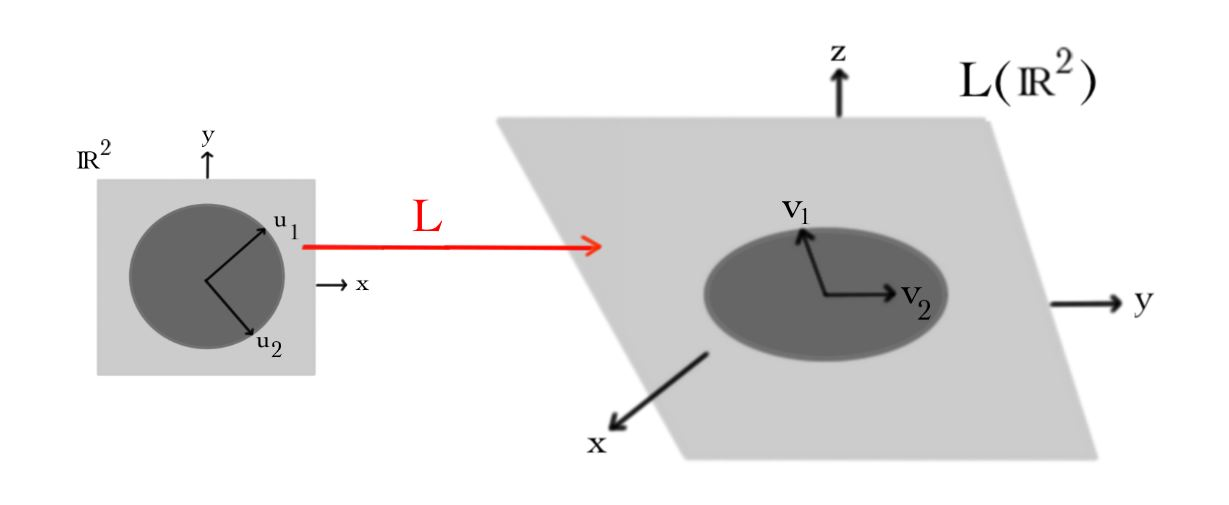
\includegraphics[scale=.27]{singval.jpg}
\end{center} 



%{\itshape Congratulations, you have reached the end of these notes! You can test your skills
%on the \hyperref[sample3]{sample final exam}.}
\begin{center}
\shabox{
{\bfseries \hyperref[sample3]{\begin{tabular}{c}Congratulations, you have reached the end of the book! \\[2mm]
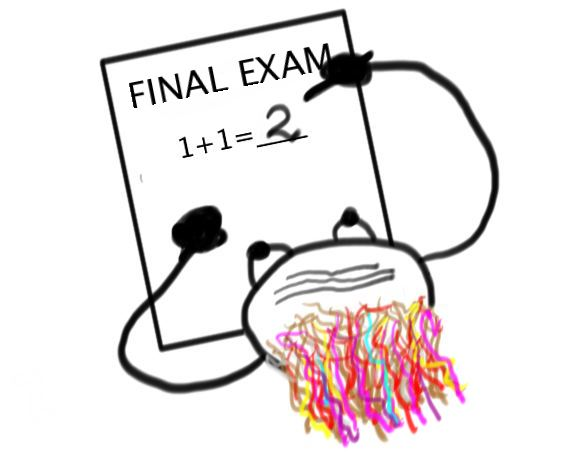
\includegraphics[scale=.15]{final.jpg}\\
Now test your skills on the \hyperref[sample3]{sample final exam}.
%You are now ready to 
%apply for membership in\\
% be a minion of Captain Conundrum's nemesis, 
%The League of Ninjas of Numbers. 
%Now test your skills
%on the sample final exam. 
\end{tabular}
}}}
\end{center}













%\section*{References}
%Hefferon, Chapter Three, Section VI.2: Gram-Schmidt Orthogonalization \\
%Beezer, Part A, Section CF, Subsection DF \\
%Wikipedia:
%\begin{itemize}
%\item \href{http://en.wikipedia.org/wiki/Linear_least_squares}{Linear Least Squares}
%\item \href{http://en.wikipedia.org/wiki/Least_squares}{Least Squares}
%\end{itemize}

\section{Review Problems}

{\bfseries Webwork:} 
\begin{tabular}{|c|c|}
\hline
Reading Problem & 
 \hwrref{LeastSquares}{1}, 
\\
   \hline
\end{tabular}






\begin{enumerate}
\item \label{det33} Let $M=\begin{pmatrix}
m^1_1 & m^1_2 & m^1_3\\
m^2_1 & m^2_2 & m^2_3\\
m^3_1 & m^3_2 & m^3_3\\
\end{pmatrix}$.  Use row operations to put $M$ into \emph{row echelon form}.  For simplicity, assume that $m_1^1\neq 0 \neq m^1_1m^2_2-m^2_1m^1_2$.

Prove that $M$ is non-singular if and only if:
\[
m^1_1m^2_2m^3_3 
- m^1_1m^2_3m^3_2 
+ m^1_2m^2_3m^3_1 
- m^1_2m^2_1m^3_3 
+ m^1_3m^2_1m^3_2
- m^1_3m^2_2m^3_1
\neq 0
\]

\phantomnewpage

\item 
\begin{enumerate}
\item What does the matrix $E^1_2=\begin{pmatrix}
0 & 1 \\
1 & 0
\end{pmatrix}$ do to $M=\begin{pmatrix}
a & b \\
d & c
\end{pmatrix}$ under left multiplication?  What about right multiplication?
\item Find elementary matrices $R^1(\lambda)$ and $R^2(\lambda)$ that respectively multiply rows $1$ and $2$ of $M$ by $\lambda$ but otherwise leave $M$ the same under left multiplication.
\item Find a matrix $S^1_2(\lambda)$ that adds a multiple $\lambda$ of row $2$ to row $1$ under left multiplication.
\end{enumerate}

\phantomnewpage

\item Let $M$ be a matrix and $S^i_jM$ the same matrix with rows \(i\) and \(j\) switched.  Explain every line of the 
\hyperlink{rowswap}{series of equations} proving that $\det M = -\det (S^i_jM)$.

\phantomnewpage

%\item \label{prob_inversion_number} This problem is a ``hands-on'' look at why \hyperlink{permutation_parity}{the property} describing the parity of permutations is true.
%
%\hypertarget{inversion_number}{The \emph{inversion number}}\index{Permutation!Inversion number} of a permutation $\sigma$ is the number of pairs $i<j$ such that $\sigma(i)>\sigma(j)$; it's the number of ``numbers that appear left of smaller numbers'' in the permutation.  For example, for the permutation $\rho = [4,2,3,1]$, the inversion number is $5$. The number $4$ comes before $2,3,$ and $1$, and $2$ and $3$ both come before $1$.
%
%Given a permutation $\sigma$, we can make a new permutation $\tau_{i,j} \sigma$ by exchanging the $i$th and $j$th entries of $\sigma$.
%
%\begin{enumerate}
%\item What is the inversion number of the permutation \(\mu=[1,2,4,3]\) that exchanges 4 and 3 and leaves everything else alone? Is it an even or an odd permutation?
%
%\item What is the inversion number of the permutation \(\rho=[4,2,3,1]\) that exchanges 1 and 4 and leaves everything else alone? Is it an even or an odd permutation?
%
%\item What is the inversion number of the permutation \(\tau_{1,3} \mu\)? Compare the parity\footnote{The \emph{parity} of an integer refers to whether the integer is even or odd. Here the parity of a permutation $\mu$ refers to the parity of its inversion number.} of \(\mu\) to the parity of \(\tau_{1,3} \mu.\)
%
%\item What is the inversion number of the permutation \(\tau_{2,4} \rho\)? Compare the parity of \(\rho\) to the parity of \(\tau_{2,4} \rho.\)
%
%\item What is the inversion number of the permutation \(\tau_{3,4} \rho\)? Compare the parity of \(\rho\) to the parity of \(\tau_{3,4} \rho.\)
%\end{enumerate}
%
%\videoscriptlink{elementary_matrices_determinant_hint.mp4}{Problem~\ref{prob_inversion_number} hints}{scripts_elementary_matrices_determinants_hint}

\phantomnewpage

%\item \label{problem_permutation} (Extra credit) Here we will examine a (very) small set of the general properties about permutations and their applications. In particular, we will show that one way to compute the sign of a permutation is by finding the \hyperlink{inversion_number}{inversion number} $N$ of $\sigma$ and we have
%\[
%\sgn(\sigma) = (-1)^N.
%\]
%
%For this problem, let $\mu = [1,2,4,3]$.
%
%\begin{enumerate}
%\item Show that every permutation $\sigma$ can be sorted by only taking simple (adjacent) transpositions\index{Permutation!Simple transposition} $s_i$ where $s_i$ interchanges the numbers in position $i$ and $i+1$ of a permutation $\sigma$ (in our other notation $s_i = \tau_{i,i+1}$). For example $s_2 \mu = [1, 4, 2, 3]$, and to sort $\mu$ we have $s_3 \mu = [1, 2, 3, 4]$.
%
%\item \label{prob_part_relations} We can compose simple transpositions together to represent a permutation (note that the sequence of compositions is not unique), and these are associative, we have an identity (the trivial permutation where the list is in order or we do nothing on our list), and we have an inverse since it is clear that $s_i s_i \sigma = \sigma$. Thus permutations of $[n]$ under composition are an example of a \hyperref[groups]{group}. However note that not all simple transpositions commute with each other since
%\begin{align*}
%s_1 s_2 [1, 2, 3] & = s_1 [1, 3, 2] = [3, 1, 2]
%\\ s_2 s_1 [1, 2, 3] & = s_2 [2, 1, 3] = [2, 3, 1]
%\end{align*}
%(you will prove here when simple transpositions commute). When we consider our initial permutation to be the trivial permutation $e = [1, 2, \dotsc, n]$, we do not write it; for example $s_i \equiv s_i e$ and $\mu = s_3 \equiv s_3 e$. This is analogous to not writing 1 when multiplying. Show that $s_i s_i = e$ (in shorthand $s_i^2 = e$), $s_{i+1} s_i s_{i+1} = s_i s_{i+1} s_i$ for all $i$, and $s_i$ and $s_j$ commute for all $|i - j| \geq 2$.
%
%\item Show that every way of expressing $\sigma$ can be obtained from using the relations proved in part~\ref{prob_part_relations}. In other words, show that for any expression $w$ of simple transpositions representing the trivial permutation $e$, using the proved relations.
%
%\emph{Hint: Use induction on $n$. For the induction step, follow the path of the $(n+1)$-th strand by looking at $s_n s_{n-1} \cdots s_k s_{k\pm1} \cdots s_n$ and argue why you can write this as a subexpression for any expression of $e$. Consider using diagrams of these paths to help.}
%
%\item The simple transpositions \hyperlink{action}{acts on} an $n$-dimensional vector space $V$ by $s_i v = E^i_{i+1} v$ (where $E^i_j$ is \hyperlink{elem_matrix_row_swap}{an elementary matrix}) for all vectors $v \in V$. Therefore we can just represent a permutation $\sigma$ as the matrix $M_{\sigma}$\footnote{Often people will just use $\sigma$ for the matrix when the context is clear.}, and we have $\det(M_{s_i}) = \det(E^i_{i+1}) = -1$. Thus prove that $\det(M_{\sigma}) = (-1)^N$ where $N$ is a number of simple transpositions needed to represent $\sigma$ as a permutation. You can assume that $M_{s_i s_j} = M_{s_i} M_{s_j}$ (it is not hard to prove) and that $\det(A B) = \det(A) \det(B)$ \hyperref[detmultiplicative]{from Chapter~\ref*{elementarydeterminantsII}}.
%
%\emph{Hint: You to make sure $\det(M_{\sigma})$ is well-defined since there are infinite ways to represent $\sigma$ as simple transpositions.}
%
%\item Show that $s_{i+1} s_i s_{i+1} = \tau_{i, i+2}$, and so give one way of writing $\tau_{i, j}$ in terms of simple transpositions? Is $\tau_{i,j}$ an even or an odd permutation? What is $\det(M_{\tau_{i,j}})$? What is the inversion number of $\tau_{i,j}$?
%
%\item The minimal number of simple transpositions needed to express $\sigma$ is called the \emph{length}\index{Permutation!Length} of $\sigma$; for example the length of $\mu$ is 1 since $\mu = s_3$. Show that the length of $\sigma$ is equal to the inversion number of $\sigma$.
%
%\emph{Hint: Find an procedure which gives you a new permutation $\sigma^{\prime}$ where $\sigma = s_i \sigma^{\prime}$ for some $i$ and the inversion number for $\sigma^{\prime}$ is 1 less than the inversion number for $\sigma$.}
%
%\item Show that $(-1)^N = \sgn(\sigma) = \det(M_{\sigma})$, where $\sigma$ is a permutation with $N$ inversions. Note that this immediately implies that $\sgn(\sigma \rho) = \sgn(\sigma) \sgn(\rho)$ for any permutations $\sigma$ and $\rho$.
%\end{enumerate}

\item Let $M'$ be the matrix obtained from $M$ by swapping two columns $i$ and $j$. Show that $\det M'=-\det M $.

\item The scalar triple product of three vectors $u,v,w$ from $\Re^3$ is $u\cdot(v\times w)$. Show that this product is the same as the determinant of the matrix whose columns are $u,v,w$ (in that order). What happens to the scalar triple product when the factors are permuted? 

\item Show that if $M$ is a $3\times 3$ matrix whose third row is a sum of multiples of the other rows ($R_3=aR_2+bR_1$) then $\det M=0$. Show that the same is true if one of the columns is a sum of multiples of the others. 

\end{enumerate}

\phantomnewpage


\newpage
